\section{Performance}\label{s:peval}

All performance tests were conducted using a desktop PC in California
with a DSL link to the Internet (\Mbps{5.6} down, \Mbps{0.7} up) as the
client, and a virtual host in a commercial data center in New
Jersey as the server.  During testing, the DSL link was otherwise
idle, and round-trip latency between the two machines was \msec{85}.  To
ensure that our results reflect the performance of StegoTorus itself
rather than factors beyond our control (such as the instantaneous load
on the global Tor network), we configured a private Tor network
entirely within the server host, and sourced all of the test files and
streams from an HTTP server also running on that host.

\smallskip\noindent\textbf{Steganographic Expansion:} We performed a
series of downloads of 1,000,000-byte files and measured the amount of
data actually transferred over the network by a direct HTTP
connection, Tor, StegoTorus using the chopper alone, and StegoTorus
with the \textit{HTTP} module. The results are shown in
Table~\ref{t:expansion}.  Tor itself has a small amount of overhead,
and the chopper imposes a little bit more, but HTTP steganography is
very expensive by comparison, increasing the amount of data sent
upstream by a factor of 41, and downstream by 12.  While we have not
spent much time on optimizing our encoding, an expansion factor of at
least eight (one byte per bit) is typical for modern steganography
schemes~\cite{a-stat-steg}, so we suspect that HTTP steganography
cannot be made \emph{that} much more efficient in the downstream
direction.

\begin{table}[ht!]
\centering\small
\newcommand\z{\phantom{.0}}
\begin{tabular}{lr@{\hspace{6pt}}rr@{\hspace{6pt}}r}
\toprule
&\multicolumn{2}{c}{\textbf{To server}}&%
 \multicolumn{2}{c}{\textbf{From server}}\\
&\textbf{bytes}&$\boldsymbol{\times}$&\textbf{bytes}&$\boldsymbol{\times}$\\
\midrule
Direct               &  23,643 &  1\z &  1,014,401 &  1\z \\
Tor                  &  61,162 &  2.6 &  1,075,715 &  1.1 \\
StegoTorus (chopper) &  63,061 &  2.7 &  1,084,228 &  1.1 \\
StegoTorus (HTTP)    & 966,964 & 41\z & 11,814,610 & 12\z \\
\bottomrule
\end{tabular}
\caption{Mean number of bytes transferred in each direction in order
  to download a 1,000,000-byte file directly, over Tor, and over
  StegoTorus with and without HTTP steganography.  The file was
  downloaded 32 times for each test.}
\label{t:expansion}
\end{table}

\begin{figure}[ht!]
\centering
% Created by tikzDevice version GitHub Dev on 2012-08-10 11:58:54
% !TEX encoding = UTF-8 Unicode
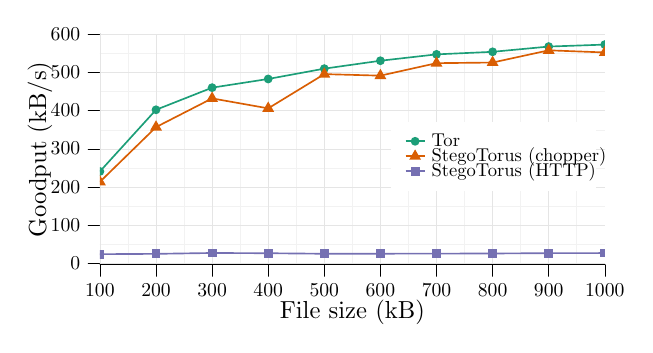
\begin{tikzpicture}[x=1pt,y=1pt]
\definecolor[named]{fillColor}{rgb}{1.00,1.00,1.00}
\begin{scope}
\definecolor[named]{drawColor}{rgb}{0.00,0.00,0.00}

\path[draw=drawColor,line width= 0.2pt,line join=round,line cap=round] ( 27.53, 22.25) -- ( 27.53,105.56);

\node[text=drawColor,anchor=base east,inner sep=0pt, outer sep=0pt, scale=  0.71] at ( 20.42, 20.48) {0};

\node[text=drawColor,anchor=base east,inner sep=0pt, outer sep=0pt, scale=  0.71] at ( 20.42, 34.29) {100};

\node[text=drawColor,anchor=base east,inner sep=0pt, outer sep=0pt, scale=  0.71] at ( 20.42, 48.09) {200};

\node[text=drawColor,anchor=base east,inner sep=0pt, outer sep=0pt, scale=  0.71] at ( 20.42, 61.89) {300};

\node[text=drawColor,anchor=base east,inner sep=0pt, outer sep=0pt, scale=  0.71] at ( 20.42, 75.70) {400};

\node[text=drawColor,anchor=base east,inner sep=0pt, outer sep=0pt, scale=  0.71] at ( 20.42, 89.50) {500};

\node[text=drawColor,anchor=base east,inner sep=0pt, outer sep=0pt, scale=  0.71] at ( 20.42,103.31) {600};
\end{scope}
\begin{scope}
\definecolor[named]{drawColor}{rgb}{0.00,0.00,0.00}

\path[draw=drawColor,line width= 0.2pt,line join=round,line cap=round] ( 23.27, 22.64) -- ( 27.53, 22.64);

\path[draw=drawColor,line width= 0.2pt,line join=round,line cap=round] ( 23.27, 36.45) -- ( 27.53, 36.45);

\path[draw=drawColor,line width= 0.2pt,line join=round,line cap=round] ( 23.27, 50.25) -- ( 27.53, 50.25);

\path[draw=drawColor,line width= 0.2pt,line join=round,line cap=round] ( 23.27, 64.05) -- ( 27.53, 64.05);

\path[draw=drawColor,line width= 0.2pt,line join=round,line cap=round] ( 23.27, 77.86) -- ( 27.53, 77.86);

\path[draw=drawColor,line width= 0.2pt,line join=round,line cap=round] ( 23.27, 91.66) -- ( 27.53, 91.66);

\path[draw=drawColor,line width= 0.2pt,line join=round,line cap=round] ( 23.27,105.47) -- ( 27.53,105.47);
\end{scope}
\begin{scope}
\path[clip] ( 27.53, 22.25) rectangle (209.98,105.56);
\definecolor[named]{drawColor}{rgb}{0.95,0.95,0.95}

\path[draw=drawColor,line width= 0.2pt,line join=round,line cap=round] ( 27.53, 29.54) --
	(209.98, 29.54);

\path[draw=drawColor,line width= 0.2pt,line join=round,line cap=round] ( 27.53, 43.35) --
	(209.98, 43.35);

\path[draw=drawColor,line width= 0.2pt,line join=round,line cap=round] ( 27.53, 57.15) --
	(209.98, 57.15);

\path[draw=drawColor,line width= 0.2pt,line join=round,line cap=round] ( 27.53, 70.96) --
	(209.98, 70.96);

\path[draw=drawColor,line width= 0.2pt,line join=round,line cap=round] ( 27.53, 84.76) --
	(209.98, 84.76);

\path[draw=drawColor,line width= 0.2pt,line join=round,line cap=round] ( 27.53, 98.57) --
	(209.98, 98.57);

\path[draw=drawColor,line width= 0.2pt,line join=round,line cap=round] ( 37.67, 22.25) --
	( 37.67,105.56);

\path[draw=drawColor,line width= 0.2pt,line join=round,line cap=round] ( 57.94, 22.25) --
	( 57.94,105.56);

\path[draw=drawColor,line width= 0.2pt,line join=round,line cap=round] ( 78.21, 22.25) --
	( 78.21,105.56);

\path[draw=drawColor,line width= 0.2pt,line join=round,line cap=round] ( 98.49, 22.25) --
	( 98.49,105.56);

\path[draw=drawColor,line width= 0.2pt,line join=round,line cap=round] (118.76, 22.25) --
	(118.76,105.56);

\path[draw=drawColor,line width= 0.2pt,line join=round,line cap=round] (139.03, 22.25) --
	(139.03,105.56);

\path[draw=drawColor,line width= 0.2pt,line join=round,line cap=round] (159.30, 22.25) --
	(159.30,105.56);

\path[draw=drawColor,line width= 0.2pt,line join=round,line cap=round] (179.57, 22.25) --
	(179.57,105.56);

\path[draw=drawColor,line width= 0.2pt,line join=round,line cap=round] (199.85, 22.25) --
	(199.85,105.56);
\definecolor[named]{drawColor}{rgb}{0.90,0.90,0.90}

\path[draw=drawColor,line width= 0.2pt,line join=round,line cap=round] ( 27.53, 22.64) --
	(209.98, 22.64);

\path[draw=drawColor,line width= 0.2pt,line join=round,line cap=round] ( 27.53, 36.45) --
	(209.98, 36.45);

\path[draw=drawColor,line width= 0.2pt,line join=round,line cap=round] ( 27.53, 50.25) --
	(209.98, 50.25);

\path[draw=drawColor,line width= 0.2pt,line join=round,line cap=round] ( 27.53, 64.05) --
	(209.98, 64.05);

\path[draw=drawColor,line width= 0.2pt,line join=round,line cap=round] ( 27.53, 77.86) --
	(209.98, 77.86);

\path[draw=drawColor,line width= 0.2pt,line join=round,line cap=round] ( 27.53, 91.66) --
	(209.98, 91.66);

\path[draw=drawColor,line width= 0.2pt,line join=round,line cap=round] ( 27.53,105.47) --
	(209.98,105.47);

\path[draw=drawColor,line width= 0.2pt,line join=round,line cap=round] ( 27.53, 22.25) --
	( 27.53,105.56);

\path[draw=drawColor,line width= 0.2pt,line join=round,line cap=round] ( 47.81, 22.25) --
	( 47.81,105.56);

\path[draw=drawColor,line width= 0.2pt,line join=round,line cap=round] ( 68.08, 22.25) --
	( 68.08,105.56);

\path[draw=drawColor,line width= 0.2pt,line join=round,line cap=round] ( 88.35, 22.25) --
	( 88.35,105.56);

\path[draw=drawColor,line width= 0.2pt,line join=round,line cap=round] (108.62, 22.25) --
	(108.62,105.56);

\path[draw=drawColor,line width= 0.2pt,line join=round,line cap=round] (128.89, 22.25) --
	(128.89,105.56);

\path[draw=drawColor,line width= 0.2pt,line join=round,line cap=round] (149.17, 22.25) --
	(149.17,105.56);

\path[draw=drawColor,line width= 0.2pt,line join=round,line cap=round] (169.44, 22.25) --
	(169.44,105.56);

\path[draw=drawColor,line width= 0.2pt,line join=round,line cap=round] (189.71, 22.25) --
	(189.71,105.56);

\path[draw=drawColor,line width= 0.2pt,line join=round,line cap=round] (209.98, 22.25) --
	(209.98,105.56);
\definecolor[named]{drawColor}{rgb}{0.11,0.62,0.47}

\path[draw=drawColor,line width= 0.6pt,line join=round] ( 27.53, 55.93) --
	( 47.81, 78.21) --
	( 68.08, 86.21) --
	( 88.35, 89.35) --
	(108.62, 93.08) --
	(128.89, 95.94) --
	(149.17, 98.24) --
	(169.44, 99.16) --
	(189.71,101.06) --
	(209.98,101.77);
\definecolor[named]{drawColor}{rgb}{0.85,0.37,0.01}

\path[draw=drawColor,line width= 0.6pt,line join=round] ( 27.53, 52.17) --
	( 47.81, 71.95) --
	( 68.08, 82.33) --
	( 88.35, 78.73) --
	(108.62, 91.10) --
	(128.89, 90.55) --
	(149.17, 95.06) --
	(169.44, 95.29) --
	(189.71, 99.70) --
	(209.98, 98.93);
\definecolor[named]{drawColor}{rgb}{0.46,0.44,0.70}

\path[draw=drawColor,line width= 0.6pt,line join=round] ( 27.53, 26.04) --
	( 47.81, 26.16) --
	( 68.08, 26.47) --
	( 88.35, 26.38) --
	(108.62, 26.19) --
	(128.89, 26.22) --
	(149.17, 26.23) --
	(169.44, 26.29) --
	(189.71, 26.40) --
	(209.98, 26.44);
\definecolor[named]{fillColor}{rgb}{0.11,0.62,0.47}

\path[fill=fillColor] ( 27.53, 55.93) circle (  1.60);

\path[fill=fillColor] ( 47.81, 78.21) circle (  1.60);

\path[fill=fillColor] ( 68.08, 86.21) circle (  1.60);

\path[fill=fillColor] ( 88.35, 89.35) circle (  1.60);

\path[fill=fillColor] (108.62, 93.08) circle (  1.60);

\path[fill=fillColor] (128.89, 95.94) circle (  1.60);

\path[fill=fillColor] (149.17, 98.24) circle (  1.60);

\path[fill=fillColor] (169.44, 99.16) circle (  1.60);

\path[fill=fillColor] (189.71,101.06) circle (  1.60);

\path[fill=fillColor] (209.98,101.77) circle (  1.60);
\definecolor[named]{fillColor}{rgb}{0.85,0.37,0.01}

\path[fill=fillColor] ( 27.53, 54.65) --
	( 29.69, 50.92) --
	( 25.38, 50.92) --
	cycle;

\path[fill=fillColor] ( 47.81, 74.44) --
	( 49.96, 70.71) --
	( 45.65, 70.71) --
	cycle;

\path[fill=fillColor] ( 68.08, 84.82) --
	( 70.23, 81.09) --
	( 65.92, 81.09) --
	cycle;

\path[fill=fillColor] ( 88.35, 81.22) --
	( 90.50, 77.49) --
	( 86.19, 77.49) --
	cycle;

\path[fill=fillColor] (108.62, 93.59) --
	(110.78, 89.85) --
	(106.47, 89.85) --
	cycle;

\path[fill=fillColor] (128.89, 93.04) --
	(131.05, 89.30) --
	(126.74, 89.30) --
	cycle;

\path[fill=fillColor] (149.17, 97.55) --
	(151.32, 93.81) --
	(147.01, 93.81) --
	cycle;

\path[fill=fillColor] (169.44, 97.78) --
	(171.59, 94.05) --
	(167.28, 94.05) --
	cycle;

\path[fill=fillColor] (189.71,102.18) --
	(191.86, 98.45) --
	(187.55, 98.45) --
	cycle;

\path[fill=fillColor] (209.98,101.42) --
	(212.14, 97.69) --
	(207.83, 97.69) --
	cycle;
\definecolor[named]{fillColor}{rgb}{0.46,0.44,0.70}

\path[fill=fillColor] ( 25.93, 24.44) --
	( 29.13, 24.44) --
	( 29.13, 27.64) --
	( 25.93, 27.64) --
	cycle;

\path[fill=fillColor] ( 46.20, 24.56) --
	( 49.41, 24.56) --
	( 49.41, 27.76) --
	( 46.20, 27.76) --
	cycle;

\path[fill=fillColor] ( 66.48, 24.87) --
	( 69.68, 24.87) --
	( 69.68, 28.07) --
	( 66.48, 28.07) --
	cycle;

\path[fill=fillColor] ( 86.75, 24.78) --
	( 89.95, 24.78) --
	( 89.95, 27.98) --
	( 86.75, 27.98) --
	cycle;

\path[fill=fillColor] (107.02, 24.59) --
	(110.22, 24.59) --
	(110.22, 27.79) --
	(107.02, 27.79) --
	cycle;

\path[fill=fillColor] (127.29, 24.62) --
	(130.49, 24.62) --
	(130.49, 27.83) --
	(127.29, 27.83) --
	cycle;

\path[fill=fillColor] (147.56, 24.63) --
	(150.77, 24.63) --
	(150.77, 27.83) --
	(147.56, 27.83) --
	cycle;

\path[fill=fillColor] (167.84, 24.69) --
	(171.04, 24.69) --
	(171.04, 27.89) --
	(167.84, 27.89) --
	cycle;

\path[fill=fillColor] (188.11, 24.80) --
	(191.31, 24.80) --
	(191.31, 28.00) --
	(188.11, 28.00) --
	cycle;

\path[fill=fillColor] (208.38, 24.84) --
	(211.58, 24.84) --
	(211.58, 28.04) --
	(208.38, 28.04) --
	cycle;
\end{scope}
\begin{scope}
\definecolor[named]{drawColor}{rgb}{0.00,0.00,0.00}

\path[draw=drawColor,line width= 0.2pt,line join=round,line cap=round] ( 27.53, 22.25) -- (209.98, 22.25);

\node[text=drawColor,anchor=base,inner sep=0pt, outer sep=0pt, scale=  0.71] at ( 27.53, 10.82) {100};

\node[text=drawColor,anchor=base,inner sep=0pt, outer sep=0pt, scale=  0.71] at ( 47.81, 10.82) {200};

\node[text=drawColor,anchor=base,inner sep=0pt, outer sep=0pt, scale=  0.71] at ( 68.08, 10.82) {300};

\node[text=drawColor,anchor=base,inner sep=0pt, outer sep=0pt, scale=  0.71] at ( 88.35, 10.82) {400};

\node[text=drawColor,anchor=base,inner sep=0pt, outer sep=0pt, scale=  0.71] at (108.62, 10.82) {500};

\node[text=drawColor,anchor=base,inner sep=0pt, outer sep=0pt, scale=  0.71] at (128.89, 10.82) {600};

\node[text=drawColor,anchor=base,inner sep=0pt, outer sep=0pt, scale=  0.71] at (149.17, 10.82) {700};

\node[text=drawColor,anchor=base,inner sep=0pt, outer sep=0pt, scale=  0.71] at (169.44, 10.82) {800};

\node[text=drawColor,anchor=base,inner sep=0pt, outer sep=0pt, scale=  0.71] at (189.71, 10.82) {900};

\node[text=drawColor,anchor=base,inner sep=0pt, outer sep=0pt, scale=  0.71] at (209.98, 10.82) {1000};
\end{scope}
\begin{scope}
\definecolor[named]{drawColor}{rgb}{0.00,0.00,0.00}

\path[draw=drawColor,line width= 0.2pt,line join=round,line cap=round] ( 27.53, 17.99) -- ( 27.53, 22.25);

\path[draw=drawColor,line width= 0.2pt,line join=round,line cap=round] ( 47.81, 17.99) -- ( 47.81, 22.25);

\path[draw=drawColor,line width= 0.2pt,line join=round,line cap=round] ( 68.08, 17.99) -- ( 68.08, 22.25);

\path[draw=drawColor,line width= 0.2pt,line join=round,line cap=round] ( 88.35, 17.99) -- ( 88.35, 22.25);

\path[draw=drawColor,line width= 0.2pt,line join=round,line cap=round] (108.62, 17.99) -- (108.62, 22.25);

\path[draw=drawColor,line width= 0.2pt,line join=round,line cap=round] (128.89, 17.99) -- (128.89, 22.25);

\path[draw=drawColor,line width= 0.2pt,line join=round,line cap=round] (149.17, 17.99) -- (149.17, 22.25);

\path[draw=drawColor,line width= 0.2pt,line join=round,line cap=round] (169.44, 17.99) -- (169.44, 22.25);

\path[draw=drawColor,line width= 0.2pt,line join=round,line cap=round] (189.71, 17.99) -- (189.71, 22.25);

\path[draw=drawColor,line width= 0.2pt,line join=round,line cap=round] (209.98, 17.99) -- (209.98, 22.25);
\end{scope}
\begin{scope}
\definecolor[named]{drawColor}{rgb}{0.00,0.00,0.00}

\node[text=drawColor,anchor=base,inner sep=0pt, outer sep=0pt, scale=  0.89] at (118.76,  2.71) {File size (kB)};
\end{scope}
\begin{scope}
\definecolor[named]{drawColor}{rgb}{0.00,0.00,0.00}

\node[text=drawColor,rotate= 90.00,anchor=base,inner sep=0pt, outer sep=0pt, scale=  0.89] at (  8.11, 63.91) {Goodput (kB/s)};
\end{scope}
\begin{scope}
\definecolor[named]{fillColor}{rgb}{1.00,1.00,1.00}

\path[fill=fillColor] (132.84, 49.01) rectangle (206.85, 73.81);
\end{scope}
\begin{scope}
\definecolor[named]{drawColor}{rgb}{0.11,0.62,0.47}

\path[draw=drawColor,line width= 0.6pt,line join=round] (137.98, 66.83) -- (144.91, 66.83);
\end{scope}
\begin{scope}
\definecolor[named]{fillColor}{rgb}{0.11,0.62,0.47}

\path[fill=fillColor] (141.44, 66.83) circle (  1.60);
\end{scope}
\begin{scope}
\definecolor[named]{drawColor}{rgb}{0.85,0.37,0.01}

\path[draw=drawColor,line width= 0.6pt,line join=round] (137.98, 61.41) -- (144.91, 61.41);
\end{scope}
\begin{scope}
\definecolor[named]{fillColor}{rgb}{0.85,0.37,0.01}

\path[fill=fillColor] (141.44, 63.90) --
	(143.60, 60.16) --
	(139.29, 60.16) --
	cycle;
\end{scope}
\begin{scope}
\definecolor[named]{drawColor}{rgb}{0.46,0.44,0.70}

\path[draw=drawColor,line width= 0.6pt,line join=round] (137.98, 55.99) -- (144.91, 55.99);
\end{scope}
\begin{scope}
\definecolor[named]{fillColor}{rgb}{0.46,0.44,0.70}

\path[fill=fillColor] (139.84, 54.39) --
	(143.04, 54.39) --
	(143.04, 57.59) --
	(139.84, 57.59) --
	cycle;
\end{scope}
\begin{scope}
\definecolor[named]{drawColor}{rgb}{0.00,0.00,0.00}

\node[text=drawColor,anchor=base west,inner sep=0pt, outer sep=0pt, scale=  0.67] at (147.41, 64.80) {Tor};
\end{scope}
\begin{scope}
\definecolor[named]{drawColor}{rgb}{0.00,0.00,0.00}

\node[text=drawColor,anchor=base west,inner sep=0pt, outer sep=0pt, scale=  0.67] at (147.41, 59.38) {StegoTorus (chopper)};
\end{scope}
\begin{scope}
\definecolor[named]{drawColor}{rgb}{0.00,0.00,0.00}

\node[text=drawColor,anchor=base west,inner sep=0pt, outer sep=0pt, scale=  0.67] at (147.41, 53.96) {StegoTorus (HTTP)};
\end{scope}
\end{tikzpicture}

\caption{Mean StegoTorus (ST) and Tor goodput for \SI{100}{\kilo\byte}
  to \SI{1}{\mega\byte} file transfers.}\label{f:goodput}
\end{figure}

\smallskip\noindent\textbf{Goodput:} Expanding on the previous
experiment, we conducted more downloads of files of various sizes,
measured the time required, and computed the mean goodput (that is,
application-layer throughput) achieved in the same configurations
described earlier; the results are shown in Figure~\ref{f:goodput}.
We see that the goodput of the chopper-only configuration is
comparable to Tor, and that StegoTorus-HTTP is only able to achieve
goodput of roughly \kBps{27}, which is still about 4 times better than
a \kbps{56} modem.  Consistent with this, we have been able to use
StegoTorus-HTTP as-is for casual Web browsing; subjectively speaking,
it is noticeably slower than a direct broadband connection, but not so
slow that waiting for page loads becomes tedious.

\smallskip\noindent\textbf{Resilience:} Since StegoTorus may be used
in locations with poor connectivity, we also investigated its
performance as a function of network latency.  We used Linux's
\textit{netem} mechanism~\cite{s-netem} to vary the round-trip latency
to the StegoTorus server from \SIrange{100}{450}{\milli\second}.  For
comparison, packets from California take approximately \msec{85} to
reach New Jersey, \SIrange{120}{180}{\milli\second} to reach East Asia or
Australia, and \SIrange{300}{350}{\milli\second} to reach India or Africa.

We configured the server to generate continuous streams of data at
three different rates, thus measuring steady-state behavior, and
recorded the median bandwidth consumption over a period of 20 seconds
at each latency setting.  The results are shown in
Figure~\ref{f:resilience}.  Ideal behavior would be for each line to
be perfectly horizontal, and as close to the “Tor” line as possible.

Both Tor and StegoTorus in chopper-only mode are robust up to
\msec{450} of delay, suffering no measurable performance degradation.
The \textit{HTTP} module, however, can keep up with a \kBps{50} data
stream only at latencies below \msec{200}.  Allowing \textit{HTTP} to
use more parallel connections increases throughput at low latencies,
but does not help it keep up at high latencies.  We suspect this is
because each chopper block, which typically will only contain one or
two Tor cells, takes a full HTTP request-response pair to transfer to
the peer.  Thus we are only transferring one or two Tor cells per
round-trip cycle, despite consuming far more bandwidth.  However, we
believe that the \textit{HTTP} module can be improved to handle high
latency at least somewhat better, and plan to make this a priority for
future work.
